\documentclass[aps,pra,twocolumn,superscriptaddress,nofootinbib]{revtex4-2}
\usepackage{amsmath,amssymb,graphicx,hyperref,xcolor}
\hypersetup{colorlinks=true,linkcolor=blue!60!black,citecolor=blue!60!black,urlcolor=blue!60!black}

\newcommand{\Tr}{\mathrm{Tr}}

\begin{document}

\title{Work statistics of post-selected quantum dynamics:\\
exact two-potential structure, an attribution no-go theorem,\\ and pre-registered tests on quantum hardware}

\author{Andrew Matlock}
%\email{<dedicated contact address before submission>}
\affiliation{Independent researcher}

\date{\today}

\begin{abstract}
Post-selection reshapes the work statistics of a quantum process in an exact and structured way. For the accepted-run two-point-measurement statistics of any post-selected dynamics with effective operator $C$ --- including Lloyd's post-selected model of closed timelike curves (P-CTCs), operationally identical to heralding --- we prove that the pairwise Crooks deviations factorize as $D_{ij}=u_j-v_i$ into dynamics-dependent potentials $u_j=\ln\lVert C^\dagger|j\rangle\rVert^2$, $v_i=\ln\lVert C|i\rangle\rVert^2$, with nonzero zero-work deviations if and only if $C$ is non-normal; the accepted-run initial marginal is biased relative to the preparation ensemble, and the Jarzynski functional is a known-type constant efficacy. A constructive no-go theorem shows that a Halmos-dilated heralded device reproduces every accepted-run statistic of a P-CTC, so such statistics cannot attribute post-selection to any particular selector; only the discard count could. We map the forgery class (single-potential generalized detailed balance, $D_{ii}=0$), show that the adjoint-reversal convention factorizes every channel --- so a detection claim must certify its reverse protocol --- and find numerically that Deutsch-model CTCs do not factorize on identical circuits, a work-statistics discriminator between the two CTC models. On two IBM Heron-r2 processors we demonstrate the two-potential structure under pre-registered, hash-committed criteria (variance explained $0.977$ and $0.989$; correlation with the parameter-free prediction $0.989$ and $0.994$; cross-device $0.981$, fully out of sample), demonstrate the biased marginal, and characterize the structure's fragility to incoherent noise. A registered, drift-immune paired test --- a normal-operator control and the non-normal circuit as sixteen circuits in a single job on the same qubits --- confirms the taxonomy on hardware: zero-work witness ratio $4.6$ and antisymmetry ratio $5.6$ against gates of $3$ and $1.5$, with the control landing in the single-potential class; two earlier absolute-gated control attempts failed to calibration drift and are reported. All registrations, raw counts, and code are provided.
\end{abstract}

\maketitle

\section{Introduction}
When histories are selected---by an experimenter's herald, a filtering archive, or a global consistency condition of the Lloyd post-selected-teleportation type~\cite{lloyd2011prl,lloyd2011pra}---the selection leaves a trace in ordinary statistics. This paper characterizes that trace exactly for the two standard quantum models of chronology violation, establishes what it cannot reveal about the selector, and tests every prediction on hardware. Fluctuation theorems~\cite{jarzynski1997,crooks1999,talknerlutzhanggi2007,seifert2012} are the natural instrument: they constrain the ratio of forward to time-reversed transition probabilities in a manner that ordinary open-system dynamics respects and selection generically breaks.

The neighboring literature is dense, and we position our claims within it precisely. That post-selection biases probabilities ``before'' the selecting element exists is anticipated qualitatively by Hartle~\cite{hartle1994} and quantitatively by Brun and Wilde~\cite{brunwilde2012}, whose reweighted-prior formula is the ancestor of our biased initial marginal. Acceptance-ratio Jarzynski equalities are a known type: classically in extended fluctuation relations~\cite{junier2009}, in feedback efficacy~\cite{sagawaueda2010}, in {\AA}berg's conditional fluctuation theorems~\cite{aberg2018}, in operator form essentially identical to ours for no-click non-Hermitian trajectories~\cite{malakarsilva2025}, and---while this work was in preparation---for the entropy production of post-selected non-Hermitian dynamics, where the reverse protocol yields a Crooks relation with a constant normalization-ratio offset tied to non-normality~\cite{cavina2026}. We accordingly claim no novelty for the efficacy result, Theorem~1(d). Two-potential deviations from the Crooks relation also exist---in {\AA}berg's framework the herald-conditioned deviation is a difference of \emph{boundary} potentials $\ln Z(Q^f)-\ln Z(Q^i)$~\cite{aberg2018}, channel fluctuation theorems carry Hamiltonian-dependent corrections of similar shape~\cite{kwonkim2019,albash2013,rastegin2014,maeda2023}, and the measurement-and-feedback fluctuation theorems of Potts, Samuelsson, and Prech~\cite{pottssamuelsson2018,prechpotts2024} produce per-\emph{record} deviations that are global log-probability ratios, as do record-conditioned theorems under imperfect detection~\cite{ferricortes2025} and trajectory-level bounds on apparent second-law violations~\cite{salazar2026}. Nearest in structure, from the measurement arrow-of-time literature, are fluctuation theorems for continuous monitoring whose boundary terms are logarithms of record success probabilities~\cite{manikandan2019} --- the ingredient of our potentials, there without post-selected TPM pairs or the acceptance renormalization that generates them. What we have not found anywhere, after a systematic sweep of the twenty-two closest papers and the full citation trees of Refs.~\cite{aberg2018,albash2013} (224 citing papers screened; documented in the repository), is the conjunction that constitutes Theorem~1: a \emph{per-pair} factorization of the normalized accepted-run Crooks deviation into potentials that are \emph{operator norms of the effective dynamics itself}, with the zero-work witness $D_{ii}\neq 0\iff C$ non-normal. The sub-normalized version of Theorem~1 sits at corollary distance from {\AA}berg's global relation and inside the Prech--Potts umbrella; the normalized, dynamics-potential form and its consequences appear to be new, and we present them as a sharpening of those frameworks. The gap is closing from both sides: the per-input-renormalized conditionals of Theorem~1(a) have been measured for non-Hermitian dynamics on a superconducting qubit~\cite{erdamar2024} and, very recently, in a trapped ion~\cite{nhje2026}---in both cases without the reverse protocol---while Ref.~\cite{cavina2026} has the reverse protocol but renormalizes globally, which collapses the per-pair structure to a single constant. The two lines of work appear unaware of each other; the present paper connects them. The attribution no-go (Theorem~2) makes constructive and statistically complete an equivalence that is folklore at the level of models---P-CTC dynamics \emph{is} postselected teleportation~\cite{lloyd2011pra,brunwilde2017sim}---and the work-statistics discriminator between Deutsch~\cite{deutsch1991} and Lloyd CTCs --- proven analytically for an explicit circuit, under both mixed-input conventions --- appears to be a new axis of comparison, complementary to the known information-theoretic~\cite{brunwilde2012,blss2009} and entropic~\cite{bartkiewicz2019} separations.

\section{Setup}
System $S$ with Hamiltonian eigenbasis $\{|i\rangle\}$, energies $E_i$, inverse temperature $\beta$; $\Delta F=0$ throughout (identical initial and final Hamiltonians). A chronology-violating register interacts with $S$ via a unitary $U$; the P-CTC prescription~\cite{lloyd2011prl,lloyd2011pra} assigns the effective, generally non-unitary operator $C=\Tr_{\rm CTC}(U)$. The TPM protocol~\cite{talknerlutzhanggi2007}: prepare the Gibbs state, projectively measure energy (outcome $i$), evolve, measure again (outcome $j$); work $W=E_j-E_i$. The reverse process uses $U^\dagger$, hence $C^\dagger$ (the physical-inverse instance of quantum operation time reversal~\cite{crooks2008reversal}; the choice of reverse map is load-bearing, cf.~Sec.~\ref{sec:forgery}). The pairwise Crooks deviation is
\begin{equation}
D_{ij}\;\equiv\;\ln\!\frac{p_{\rm th}(i)\,p(j|i)}{p_{\rm th}(j)\,\tilde p(i|j)}\;-\;\beta W_{ij}
\;=\;\ln\frac{p(j|i)}{\tilde p(i|j)},
\label{eq:Ddef}
\end{equation}
where the second equality uses $\Delta F=0$. For ordinary unitary dynamics $D_{ij}=0$ (the Crooks relation); nonzero entries of $D$ are the object of study.

\section{Theorem 1: the structure of the P-CTC TPM joint}
\textbf{Statement.} Assume $\lVert C|i\rangle\rVert>0$ and $\lVert C^\dagger|j\rangle\rVert>0$ for all $i,j$ (an input with $C|i\rangle=0$ is never accepted and its row drops out; Appendix~\ref{app:derivation}); degeneracies generalize with subspace-trace potentials. Model the first measurement by an explicit record register $M$ (the energy index is copied unitarily into $M$ before the CTC interaction; $M$ never touches the CTC). Applying the P-CTC rule once to the full circuit yields the joint
\begin{equation}
P(i,j)=\frac{p_{\rm th}(i)\,|\langle j|C|i\rangle|^2}{N_F},\qquad
N_F=\sum_k p_{\rm th}(k)\,\lVert C|k\rangle\rVert^2 .
\label{eq:joint}
\end{equation}
Consequently:
\emph{(a)} the conditionals are per-input renormalized, $p(j|i)=|\langle j|C|i\rangle|^2/\lVert C|i\rangle\rVert^2$;
\emph{(b)} with $u_j=\ln\lVert C^\dagger|j\rangle\rVert^2$ and $v_i=\ln\lVert C|i\rangle\rVert^2$,
\begin{equation}
\boxed{\;D_{ij}=u_j-v_i\;}
\label{eq:factorization}
\end{equation}
exactly---an all-pairs factorization into two state potentials; since $|\langle i|C^\dagger|j\rangle|=|\langle j|C|i\rangle|$ identically, no transition can vanish one-sidedly (no ``quantum amputation'' of the spectrum);
\emph{(c)} the \emph{initial-outcome marginal} is biased,
$P(i)=p_{\rm th}(i)\lVert C|i\rangle\rVert^2/N_F\neq p_{\rm th}(i)$,
a measurable deviation of the past from the verified preparation with zero discarded runs (quantitatively this is the Brun--Wilde reweighted prior~\cite{brunwilde2012} in a thermal TPM setting);
\emph{(d)} $\langle e^{-\beta W}\rangle=N_R/N_F$ with $N_R=\sum_k p_{\rm th}(k)\lVert C^\dagger|k\rangle\rVert^2$: a constant efficacy of the feedback type, independently established in several lineages~\cite{sagawaueda2010,aberg2018,junier2009,malakarsilva2025,cavina2026}. Parts (a) and (b) involve only per-input renormalization and are independent of the global-versus-per-branch prescription choice that afflicts nonlinear theories; parts (c) and (d) use the global rule, whose justification --- and the per-branch alternative --- are given in Appendix~\ref{app:derivation}.

\textbf{Proof.} Appendix~\ref{app:derivation}. In brief: Eq.~\eqref{eq:joint} follows from applying the prescription once to the recorded circuit; for (b), $\tilde p(i|j)=|\langle i|C^\dagger|j\rangle|^2/\lVert C^\dagger|j\rangle\rVert^2$ and the numerators cancel in~\eqref{eq:Ddef}. All four statements are additionally verified numerically to $\sim10^{-16}$, including an independent construction of $C$ from explicit postselected-teleportation amplitudes. $\square$

Three remarks. First, the potentials in~\eqref{eq:factorization} are norms of the \emph{dynamics}, not of boundary operators: this is what distinguishes Eq.~\eqref{eq:factorization} from the boundary-potential deviations of conditional fluctuation theorems~\cite{aberg2018,kwonkim2019} and from classical branch free energies~\cite{junier2009}. Second, the zero-work diagonal is the witness: $D_{ii}=u_i-v_i\neq 0$ is possible if and only if $C$ is non-normal, and no reference-equilibrium explanation can reproduce it (Sec.~\ref{sec:forgery}). Third, the relation to Ref.~\cite{cavina2026}: there the renormalized Crooks relation for post-selected non-Hermitian dynamics carries a single \emph{constant} offset $\Xi=\ln\mathcal{N}-\ln\tilde{\mathcal{N}}$, because the renormalization is global and the reverse prior is the evolved state; Eq.~\eqref{eq:factorization} is what that constant unfolds into under accepted-run (per-input) renormalization with thermal priors---the per-pair resolution is exactly the information the global treatment integrates out. Relatedly, Ref.~\cite{nhje2026} identifies symmetry conditions under which the conditional Jarzynski equality holds exactly --- in the language of (d), regimes where the efficacy equals unity.

\section{Theorem 2: attribution no-go, constructive}
\textbf{Statement.} For any P-CTC operator $C$, let $K=C/\lVert C\rVert$ and let $V$ be its Halmos unitary dilation~\cite{sznagy2010}. The heralded protocol (ancilla $|0\rangle$, apply $V$, accept on ancilla outcome $0$) reproduces the P-CTC's forward conditionals, reverse conditionals, and biased initial marginal \emph{exactly}. Hence, for a single use of the device with the stated input ensembles, no accepted-run TPM statistic distinguishes a P-CTC from an ordinary post-selected device; the unique distinguishing observable is the discard count (the heralded device rejects runs; the CTC rejects none). Discard-free selection is thus a nonlinearity witness in principle---but certifying it requires knowing the total number of trials: the denominator of history.

\textbf{Proof.} $\langle j|K|i\rangle\propto\langle j|C|i\rangle$ with an $i$-independent constant that cancels in every renormalized quantity; dilation existence is Sz.-Nagy/Halmos. Verified to $\sim10^{-16}$. $\square$

The model-level equivalence P-CTC $\equiv$ postselected teleportation is standard~\cite{lloyd2011pra,brunwilde2017sim}, and Lloyd and Preskill reached a kindred unattributability conclusion for black-hole final-state projection~\cite{horowitzmaldacena2004} by complexity arguments~\cite{lloydpreskill2014}. What Theorem~2 adds is the constructive dilation for arbitrary $C$ and the completeness of the equivalence across TPM observables \emph{including the biased marginal}, reducing attribution to a single number no archive carries. (The energetics of post-selection are themselves nontrivial---any nontrivial post-selection confers unbounded work benefit~\cite{purvesshort2021}---which makes the statistical unattributability the more consequential.) In archival or cosmological settings the denominator is unobtainable in principle. The theorem's scope should be stated plainly: it covers single-use TPM observables under the global prescription; nonlinear dynamics can in general be probed further by proper- versus improper-mixture inputs~\cite{blss2009}, or by composing and adaptively reusing the nonlinearity --- resources that archival statistics likewise do not provide. Theorem~2 is also what licenses the experiments of Sec.~\ref{sec:hardware}: a heralded circuit measures P-CTC statistics \emph{exactly}, so every prediction of Theorem~1 is testable on present-day processors.

\section{The forgery class and the role of the reverse protocol}
\label{sec:forgery}
Any process satisfying generalized detailed balance with respect to a reference distribution $q$---$q_i\,p(j|i)=q_j\,\tilde p(i|j)$---has $D_{ij}=\ln(q_j/q_i)$: exactly separable, but with a \emph{single} potential, hence antisymmetric with $D_{ii}=0$. A bath at the wrong temperature realizes this exactly (verified: residual $9\times10^{-16}$ at mean violation $0.53$). Therefore: (i) factorization alone is \emph{necessary, not sufficient} for post-selected consistency; (ii) the sub-signature that excludes every reference equilibrium, generalized Gibbs ensembles included, is the two-potential structure $u\neq v$, equivalently nonzero deviations at zero work, $D_{ii}\neq0$; (iii) mundane heralded operations share the two-potential structure (they \emph{are} renormalized single-operator statistics), consistent with Theorem~2: the taxonomy bottoms out at post-selection-of-any-origin.

\emph{The taxonomy of TPM Crooks deviations.} Non-separable $\rightarrow$ generic driven open dynamics. Separable with a single potential ($D_{ii}=0$) $\rightarrow$ reference equilibrium of some kind. Separable with two potentials ($D_{ii}\neq0$) $\rightarrow$ post-selection of some origin; further attribution is impossible without trial accounting (Theorem~2). The first two arrows are exact; the attribution reading of the third is an inference supported over the channel ensembles tested here, not a theorem --- constrained adversarial channels approach the class boundary.

\emph{A convention caveat discovered in audit.} The taxonomy presumes the \emph{physical-inverse} reverse protocol: run the inverse dynamics with a fresh environment, as our hardware does. The choice of reverse process is foundational rather than conventional~\cite{buscemiscarani2021}, and here it is load-bearing: under adjoint reversal with per-input renormalization, the single matrix $\sum_a|K_a[j,i]|^2$ read column-normalized is the forward conditional and read row-normalized is the reverse conditional, so \emph{every} channel factorizes exactly (verified to $7\times10^{-16}$ over random channels). A detection claim must therefore certify its reverse protocol and test factorization \emph{into the predicted, dynamics-dependent potentials}---which no convention artifact and no reference equilibrium reproduces. Under the physical-inverse protocol, random dilation channels with genuine violations never factorize (minimum residual $0.40$, medians $0.94$--$1.30$ over $300$ draws), while adversarially constrained channels can approach it ($0.054$), so robustness claims are ensemble-dependent.

The classical analogue of these phenomena lives inside the absolute-irreversibility framework~\cite{murashita2014,funo2017,murashita2017feedback,manzano2024}: in an exactly enumerated driven Markov ring, reversal-symmetric closure ($x_T=x_0$) preserves the detailed fluctuation theorem exactly, while information-carrying twisted constraints ($x_0=x_T+k$) amputate the mirror branch of the entropy-production spectrum entirely. Quantum coherence forbids the amputation (Theorem~1b) and replaces it with the factorization~\eqref{eq:factorization}. Our residual contribution to that story is the symmetry classification: \emph{reversal-symmetric consistency is thermodynamically free; only twisted retro-constraints register}.

\section{A work-statistics discriminator between Deutsch and Lloyd CTCs}
On identical Haar-random circuits, computing Deutsch-model~\cite{deutsch1991} statistics via the fixed point $\tau=\Tr_S[U(\rho\otimes\tau)U^\dagger]$ per measured branch: D-CTC deviations are strongly non-separable (residuals $0.27$--$0.42$, comparable to the deviations themselves), while Lloyd deviations factorize to machine precision.

\emph{Proposition (analytic separation).} For a two-level system, separability $D_{ij}=u_j-v_i$ is equivalent to the vanishing of the cycle invariant $\Sigma\equiv D_{00}+D_{11}-D_{01}-D_{10}$, and every P-CTC has $\Sigma=0$ identically by Theorem~1. For the explicit circuit $U_0=e^{-i\pi\,\mathrm{SWAP}/4}\,\bigl(R_y(\tfrac{\pi}{2})\otimes\openone\bigr)\,\mathrm{CR}_y(\tfrac{\pi}{2})$ on one system and one CTC qubit, the Deutsch model gives --- in exact symbolic arithmetic, with a \emph{unique} fixed point in every branch, so no maximum-entropy tie-breaking is invoked --- rational conditionals $\bigl(p(0|0),p(0|1)\bigr)=(\tfrac12,\tfrac34)$, $\bigl(\tilde p(0|0),\tilde p(0|1)\bigr)=(\tfrac14,\tfrac58)$, hence
\begin{equation}
\Sigma_{\rm D}=\ln\tfrac{5}{3}\;\neq\;0 ,
\end{equation}
and under the rival mixture prescription (shared fixed point from the thermal input) $\Sigma_{\rm D}=\ln R_B\approx0.530\neq0$. The two CTC models are therefore separated by an exact work-statistics invariant on an explicit circuit, under \emph{both} conventions for the nonlinear theory's mixed inputs; genericity of the separation across circuits remains numerical. The two standard models of quantum time travel---already known to be inequivalent information-theoretically~\cite{brunwilde2012,blss2009} and entropically~\cite{bartkiewicz2019}---are thus also distinguishable by work-fluctuation \emph{structure}. The Haar-ensemble results likewise survive both conventions for the Bennett--Leung--Smith--Smolin mixture ambiguity~\cite{blss2009} numerically.

\section{Measurements on quantum hardware}
\label{sec:hardware}
All experiments run the heralded equivalent (Theorem~2) of a fixed shallow circuit on IBM Heron-r2 processors, with readout twirling and dynamical decoupling; all measurements, including the herald, are terminal. The effective operator and the predicted potentials are computed from the logical circuit, which the transpiled circuits realize exactly in the absence of noise; a single predicted $D$ matrix therefore gates both devices. The shallow ansatz (4 CX; transpiled depth 26, 5 two-qubit gates) was selected for high acceptance, no small transition probabilities, and strong two-potential structure ($\max|D_{ii}|=1.21$ ideal). Full protocols, job identifiers, raw counts, and analysis code are in the repository.

\subsection{Pre-registration and reproducibility}
All hardware claims in this paper were fixed in hash-committed pre-registrations before data collection, with the analysis scripts frozen; raw counts are committed to the repository in the session they are measured, and the negative control of Sec.~\ref{sec:control} was likewise registered before its data existed. A first registration (v1), whose thresholds were derived from an idealized depolarizing-noise model, returned \emph{inconclusive} by margins of $0.004$ and $0.0006$ on its two gates; we report this openly. The v2 registration replaced the noise-model-derived thresholds with device-calibrated ones (disclosed as such in the registration), corrected two statistical defects found in audit (an error model that treated the reweighted marginal as a multinomial draw rather than propagating binomial acceptance errors, and a fragile max-statistic gate sitting on a device-systematic floor), and added a second-device replication arm. The v2 criteria gate on: variance explained by~\eqref{eq:factorization} $\geq0.90$; correlation with the \emph{predicted} deviation matrix $r\geq0.95$; fitted potentials within $0.25$/$0.15$ of prediction; and, for the initial-marginal bias, acceptance-uniformity $\chi^2(3)\geq30$ with attenuation coefficient $\geq0.35$ at $\geq5\sigma$.

\subsection{The biased initial marginal}
Inputs are prepared as energy eigenstates with equal shot counts and the Gibbs weights are applied in the analysis; because the thermal state is a classical mixture diagonal in the measured basis, this reweighting is statistically equivalent to sampling the input from the Gibbs distribution, and the directly measured content of the effect is the input dependence of the herald acceptance. On a deep dilation circuit at $10^5$ shots per input --- a retrospective dataset predating the registrations, quoted as characterization --- the acceptances range from $0.146$ to $0.842$ across inputs, and the reconstructed marginal deviates from the thermal weights by $0.133$ (ideal prediction $0.146$) with zero runs discarded beyond the herald. Shot-noise-only propagation would put this at $182\sigma$, but at these counts the error budget is systematics-dominated, so we do not lean on that figure; the operative comparison is that the readout assignment errors of the measured qubits --- taken from the calibration records attached to each job --- were $0.6$--$1.0\%$ for the deep run and $0.3$--$0.5\%$ for the pre-registered arms, bounding herald-misclassification shifts of each acceptance below $0.01$, two orders of magnitude below the measured $0.70$ acceptance span. On the shallow circuit (the pre-registered arms) the contrast is smaller by design: marginal deviation $0.0115$ at $13.8\sigma$, with acceptance-contrast attenuation $0.6931\pm0.039$ ($17.8\sigma$ from zero) on ibm\_marrakesh and $0.8414$ on ibm\_fez, relative to the ideal contrast (Fig.~\ref{fig:potentials}, right). The attenuation is an empirical, device-dependent noise parameter; we do not interpret it beyond the readout bound above.

\subsection{The factorization, confirmed on two devices}
The v2 runs (one eight-circuit job per device, $2\times10^4$ shots per input) passed \emph{every} pre-registered gate on both arms. On ibm\_marrakesh (primary): variance explained $0.977$, $r(D,D^{\rm th})=0.989$, potentials within $0.149/0.093$ of prediction; initial-marginal bias confirmed as above. On ibm\_fez (replication): variance explained $0.989$, $r=0.994$; cross-device correlation of the measured deviation matrices $r=0.981$. The replication arm is fully out of sample---no data from that device entered the threshold calibration---and passed with wider margins than the primary. The fit has seven free parameters on sixteen cells; the primary statistic is the correlation with the parameter-free prediction, which is robust: leave-one-out ranges $[0.988,0.992]$ (marrakesh) and $[0.993,0.995]$ (fez), with Spearman rank correlations $0.90$ and $0.92$ (rank statistics are diluted by the deliberate clustering of the designed deviations). Figure~\ref{fig:ledger} shows the deviation matrices; Fig.~\ref{fig:potentials} the potentials. The deviation structure also replicates across seven weeks and a device-calibration era on the same processor (12 overlapping cells with an earlier partial run: $r=0.997$).

\begin{figure*}
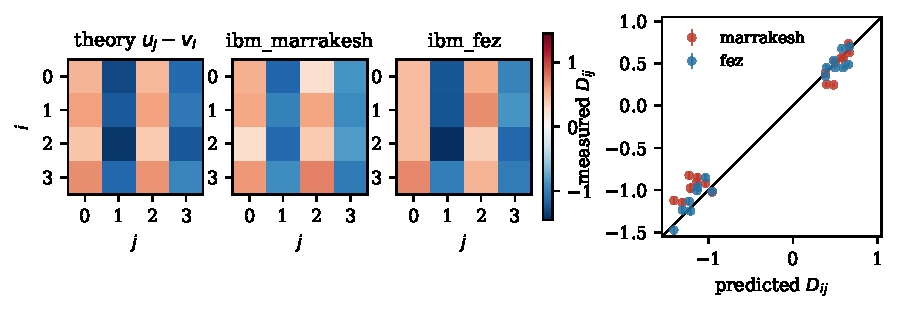
\includegraphics[width=\textwidth]{fig1_ledger.pdf}
\caption{\textbf{The two-potential structure on hardware.} Left three panels: the predicted deviation matrix $D_{ij}=u_j-v_i$ (Eq.~\ref{eq:factorization}) and the measured matrices on two Heron-r2 processors ($2\times10^4$ shots/input, all sixteen cells, pre-registered criteria). Right: measured versus predicted deviations with shot-noise error bars; the line is identity, not a fit. Variance explained: $0.977$ (marrakesh), $0.989$ (fez); cross-device $r=0.981$.}
\label{fig:ledger}
\end{figure*}

\begin{figure*}
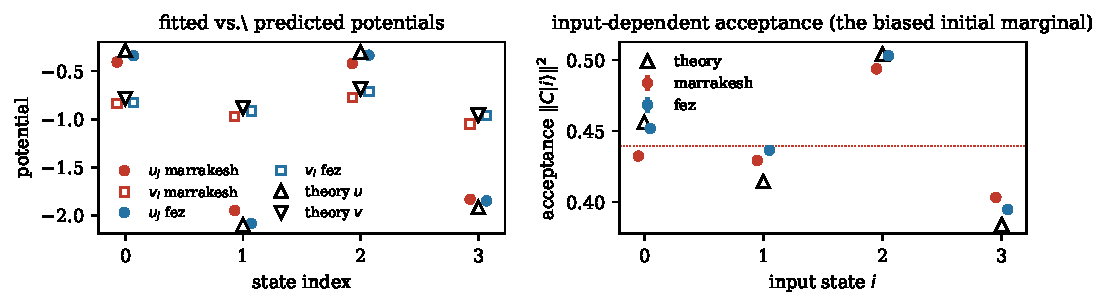
\includegraphics[width=\textwidth]{fig2_potentials.pdf}
\caption{\textbf{Potentials and the biased initial marginal.} Left: the fitted potentials $u_j$, $v_i$ (weighted least squares on the measured $D$, common gauge) against the parameter-free predictions $\ln\lVert C^\dagger|j\rangle\rVert^2$, $\ln\lVert C|i\rangle\rVert^2$. Right: measured acceptance versus input state on both devices against the ideal $\lVert C|i\rangle\rVert^2$; the input dependence \emph{is} the initial-marginal bias (acceptance-uniformity $\chi^2(3)=358$; attenuation $0.693$ at $17.8\sigma$).}
\label{fig:potentials}
\end{figure*}

\subsection{Noise fragility, and what the residual measures}
The fingerprint is destroyed by incoherent noise: on the deep circuit ($\sim20$ two-qubit gates) the separability residual saturates near $0.35$ and does not shrink with shot count. Mechanistically, a coherent error common to the forward circuit and its reversed partner merely realizes a different operator, for which Theorem~1 holds with shifted potentials; coherent errors that differ between the two separately executed circuits do contribute, so the residual bounds the incoherent fraction together with forward--reverse coherent mismatch. This is why the confirmatory statistics gate on global structure (variance explained, correlation with prediction) rather than on the maximum residual, which sits on the device-systematic floor ($0.33$--$0.40$ in all runs) at any shot count. For the detection doctrine the lesson is sharp: an archive whose records passed through a noisy channel has had the fingerprint erased; the audit requires high-fidelity records as well as complete ones.

\subsection{A same-device negative control}
\label{sec:control}
If hardware noise generically produced two-potential structure, the demonstrations above would be suspect. We therefore registered and ran a control: the same 4-CX ansatz family, with parameters optimized so the heralded block is \emph{normal} to $10^{-12}$---predicted single-potential class ($D_{ii}=0$, $D$ antisymmetric) at deviation scale comparable to the CTC circuit. Two registered attempts were made on the same processor, and we report both. The first (gates committed from noiseless simulation) fit the single-potential form with variance explained $0.961$ and $r=0.981$ against the predicted $v_j-v_i$, passing two of three gates and missing its antisymmetry gate ($0.332$ vs $\leq0.30$). The second, under re-registered gates calibrated to the measured class gap, transpiled to a different layout, caught roughly $2.3\times$ the noise, and passed one of three (single-potential variance explained $0.79$; $\max|D_{ii}|=0.303$; antisymmetry $0.74$). Under its own registered standards the control is therefore \emph{not confirmed}, and we do not claim it as one. What the two runs establish empirically is a noise floor for the witness: at this circuit's contrast, device noise produced zero-work deviations of at most $|D_{ii}|=0.303$ and antisymmetry ratios of at most $0.74$ across runs and layouts, while the non-normal circuit shows a measured $1.02$ (ideal $1.21$) and $1.37$ on the same processor---factors of $3.4$ and $1.9$ above the worst control run (Fig.~\ref{fig:control}). The acceptance profile, which encodes the operator norms, replicated closely across the control runs ($r=0.95$ on the deviation matrices); the instability lies in the low-contrast residuals, consistent with the noise-fragility mechanism above. That diagnosis --- drift and layout variance dominating absolute thresholds at low contrast --- dictated a third, differently designed registration: both arms as sixteen circuits in a \emph{single job} on the same pinned qubits with a fixed transpiler seed (one calibration snapshot; common drift cancels), a control ansatz re-optimized to normality $3\times10^{-13}$ at single-potential contrast $1.318$, and gates on \emph{paired ratios} calibrated below the historical cross-session values. The paired test passed every registered gate: zero-work witness ratio $R_D=4.55$ (gate $\geq3$), antisymmetry ratio $R_A=5.58$ (gate $\geq1.5$), with the CTC arm reproducing the factorization a fourth time (variance explained $0.969$, $r=0.980$) and the control arm landing cleanly in the single-potential class (single-potential variance explained $0.986$, $r=0.991$ against the predicted $v_j-v_i$, $\max|D_{ii}|=0.268$, antisymmetry $0.232$) --- incidentally meeting even the earlier absolute thresholds once drift was controlled (Fig.~\ref{fig:control}). The taxonomy demonstration therefore rests on a passed, registered, drift-immune gate; the two failed absolute-gated attempts stand in the record as the measurement of why absolute gates were the wrong instrument.

\begin{figure}
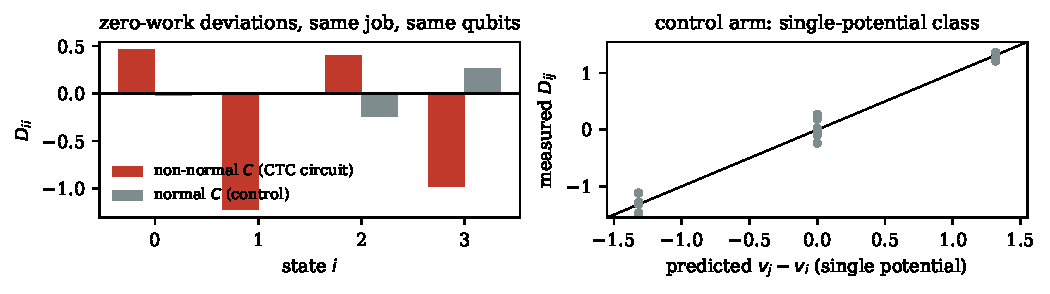
\includegraphics[width=\columnwidth]{fig3_control.pdf}
\caption{\textbf{The taxonomy on hardware, paired.} Both panels from the registered paired test: sixteen circuits in one job on the same qubits. Left: zero-work deviations $D_{ii}$ for the non-normal (CTC) arm and the normal-operator control arm; the paired witness ratio is $R_D=4.55$ against a registered gate of $3$. Right: the control arm's measured deviations against the parameter-free single-potential prediction $v_j-v_i$ (variance explained $0.986$).}
\label{fig:control}
\end{figure}

\section{Limitations}
(1) All systems are small ($\leq5$ qubits, 4 levels); single-shot TPM protocols; no thermodynamic limit. (2) The hardware experiments test Theorem~1's statistics via Theorem~2's heralded equivalence; they involve real discards at the herald and are not evidence of discard-free selection---by Theorem~2, nothing statistical could be. (3) Reverse-process conventions for the open-system null were not exhausted (Petz-type reversals untested), though the adjoint convention is now mapped and shown degenerate. (4) The Deutsch--Lloyd separation is proven for an explicit circuit under both mixed-input conventions; its genericity across circuits remains numerical, and the mixture ambiguity~\cite{blss2009} attaches to that ensemble statement. (5) The forgery-class robustness is ensemble-dependent, and constrained adversarial optimization approaches the fingerprint. (6) Two absolute-gated control attempts failed to calibration drift before the paired, ratio-gated design passed all its registered gates (Sec.~\ref{sec:control}); all three registrations and raw datasets are in the repository. (7) Priority: our systematic sweep covers the 22 closest papers, the full Semantic Scholar citation trees of Refs.~\cite{aberg2018,albash2013} (224 papers screened, $\sim$15 read in depth), the post-2024 non-Hermitian work-statistics tree, and full-text phrase searches; no statement of Eq.~\eqref{eq:factorization} was found, but the literature is dense and moving quickly---Ref.~\cite{cavina2026} appeared during preparation with the reverse protocol and the constant-offset relation---and we present Theorem~1 as a sharpening of the frameworks of Refs.~\cite{aberg2018,prechpotts2024,cavina2026} rather than an independent discovery. (8) Nothing here bears on whether CTCs exist; the paper concerns the statistics of consistency \emph{models}.

\section{Conclusion}
We have shown that post-selection imprints an exact two-potential structure on TPM work statistics (Theorem~1), verified that structure on two quantum processors under pre-registered criteria, and delimited what such statistics can support. Accepted-run statistics can display the two-potential structure characteristic of post-selection, can exclude every exact reference-equilibrium explanation through the zero-work witness $D_{ii}\neq0$, and can distinguish the Deutsch from the Lloyd model of chronology violation by separability alone. By Theorem~2 they cannot attribute the post-selection to any particular selector: the accepted-run statistics of a closed timelike curve and of an ordinary heralded filter coincide exactly, and the one discriminating observable---the discard count---is precisely what archival and cosmological observers lack, a structure familiar from the measure problem. Natural continuations include Petz-type reverse protocols for the open-system null model, quantitative bounds on adversarial forgery of the two-potential structure, larger systems, and a formal embedding of the normalized accepted-run theory in the frameworks of Refs.~\cite{aberg2018,prechpotts2024,cavina2026}. Three applications suggest themselves: the separability residual as an inexpensive witness separating incoherent from coherent device noise (Sec.~\ref{sec:hardware}); the reverse protocol and the zero-work witness $D_{ii}$ as a direct experimental probe of non-normality on non-Hermitian platforms, where the forward conditionals are already measured routinely~\cite{erdamar2024,nhje2026}; and the question of whether black-hole final-state projection~\cite{horowitzmaldacena2004,lloydpreskill2014} imprints two-potential structure on Hawking-radiation work statistics.

\emph{Reproducibility.} The repository accompanying this paper contains all pre-registrations with SHA-256 hashes committed before data, raw measurement counts for every hardware run reported (including the runs that returned inconclusive), fixed-seed analysis and simulation code, and the audit trail documenting every statistical correction made between registrations.

\begin{acknowledgments}
\emph{Provenance disclosure: this work was produced collaboratively by the human author and an AI assistant (Anthropic's Claude), spanning conjectures, proofs, code, adversarial review, and prose. The human author takes responsibility for all claims. Quantum-hardware time was provided by the IBM Quantum Open Plan.}
\end{acknowledgments}

\appendix

\section{Derivation of the joint distribution}
\label{app:derivation}
Model the first energy measurement by a record register $M$: conditioned on outcome $i$ (probability $p_{\rm th}(i)$), the system--record state is $|i\rangle_S|i\rangle_M$, and $M$ does not interact with the CTC register. The P-CTC prescription applied once to the remainder of the circuit replaces the unitary acting on $S$ (and the CTC register) by the effective operator $C=\Tr_{\rm CTC}(U)$ and renormalizes the resulting subnormalized state globally:
\begin{equation}
\rho_{SM}\;\mapsto\;\frac{(C\otimes\openone_M)\,\rho_{SM}\,(C^\dagger\otimes\openone_M)}{\Tr\!\left[(C^\dagger C\otimes\openone_M)\,\rho_{SM}\right]},
\end{equation}
with $\rho_{SM}=\sum_i p_{\rm th}(i)\,|ii\rangle\langle ii|$. Because the prescription is nonlinear, mixed inputs are prescription-sensitive~\cite{blss2009}: applying the rule separately to each pure component of the proper thermal mixture renormalizes per branch, which yields the same conditionals as (a) but an \emph{unbiased} marginal, whereas applying it once to the recorded circuit yields Eq.~\eqref{eq:joint}. We adopt the global rule for a stated reason rather than by fiat: in Lloyd's definition the P-CTC is a single postselected-teleportation event within one circuit, the record register makes the first measurement's outcome part of that circuit's physical state, and the postselection acts on the whole; under the per-branch reading the consistency filter would act separately conditioned on a record it has no access to. Symmetrically with the Deutsch-model mixture caveat of the discriminator section: Theorem~1(c) and (d) are statements about the global prescription, while (a) and (b) hold under either. Reading out $M=i$ and the final energy $j$ gives Eq.~\eqref{eq:joint} directly, with $N_F=\sum_k p_{\rm th}(k)\lVert C|k\rangle\rVert^2$ the global normalization. The reverse process is the same construction with $C^\dagger$ and yields $\tilde P(j,i)=p_{\rm th}(j)|\langle i|C^\dagger|j\rangle|^2/N_R$. The conditionals are then $p(j|i)=|\langle j|C|i\rangle|^2/\lVert C|i\rangle\rVert^2$ and $\tilde p(i|j)=|\langle i|C^\dagger|j\rangle|^2/\lVert C^\dagger|j\rangle\rVert^2$; substituting into Eq.~\eqref{eq:Ddef} and using $|\langle i|C^\dagger|j\rangle|=|\langle j|C|i\rangle|$ cancels the matrix elements and leaves $D_{ij}=u_j-v_i$. For the efficacy,
\begin{align}
\langle e^{-\beta W}\rangle
&=\sum_{ij}\frac{p_{\rm th}(i)|\langle j|C|i\rangle|^2}{N_F}\,e^{-\beta(E_j-E_i)}\nonumber\\
&=\frac{1}{N_F}\sum_j \frac{e^{-\beta E_j}}{Z}\sum_i|\langle j|C|i\rangle|^2
=\frac{N_R}{N_F},
\end{align}
using $p_{\rm th}(i)e^{\beta E_i}=1/Z$ and $\sum_i|\langle j|C|i\rangle|^2=\lVert C^\dagger|j\rangle\rVert^2$. Degeneracies require no special treatment (the basis is fixed by the measurement); if $C|i\rangle=0$ for some $i$, that input is never accepted, $v_i=-\infty$, and the corresponding row of $D$ is empty --- matching the minimum-count cell filter in the analysis. The restriction $\Delta F=0$ is for clarity only: with distinct initial and final Hamiltonians the factorization holds with $\beta\Delta F$ absorbed into the potentials.

For Theorem~2, set $K=C/\lVert C\rVert$ (operator norm) and
\begin{equation}
V=\begin{pmatrix} K & (\openone-KK^\dagger)^{1/2}\\[2pt] (\openone-K^\dagger K)^{1/2} & -K^\dagger \end{pmatrix},
\end{equation}
which is unitary (Halmos~\cite{sznagy2010}). With the ancilla prepared in $|0\rangle$ and accepted on outcome $0$, the accepted block of $V$ is $K$ and the accepted block of $V^\dagger$ is $K^\dagger$, so the reverse protocol dilates consistently. Since $\langle j|K|i\rangle=\langle j|C|i\rangle/\lVert C\rVert$ with an input-independent constant, every renormalized quantity --- forward and reverse conditionals and the marginal of Eq.~\eqref{eq:joint} --- is identical for the two devices, which proves the theorem.

\section{Statistical notes}
\label{app:stats}
Cell error bars use the delta method for a log-transformed multinomial proportion, $\mathrm{Var}[\ln\hat p]\approx(1-p)/n_{\rm cell}$, per direction. Cells within one row share a normalization and are therefore weakly anticorrelated, $\mathrm{Cov}[\ln\hat p_a,\ln\hat p_b]\approx-1/N_{\rm row}$; at the accepted counts of our runs this is one to two orders of magnitude below the cell variances and is neglected in the weighted fit --- it does not enter the confirmation gates, which use variance explained and correlation rather than $\chi^2$. Variance explained is defined as $1-\mathrm{Var}[r]/\mathrm{Var}[D]$ over used cells, with $r$ the residuals of the weighted least-squares fit of $D_{ij}=u_j-v_i$ (eight parameters, one gauge). For the biased marginal, the acceptances are four independent binomials; the marginal's covariance follows by the delta method through the normalization, and the model-free statistic is the acceptance-uniformity $\chi^2$ on three degrees of freedom.

\emph{Data availability.} All pre-registrations (with SHA-256 hashes committed to version control before data collection), raw measurement counts for every run reported including the inconclusive v1 run, analysis scripts, and simulation code are available in the accompanying repository [URL/DOI to be inserted at submission].

\bibliography{refs}

\end{document}
